\documentclass{article}
%\documentclass{exam}
\usepackage[italian]{babel}
\usepackage[T1]{fontenc}
\usepackage{graphicx}
\usepackage[utf8x]{inputenc}
\usepackage{amsmath}
\usepackage{amsthm}
\usepackage{hyperref}
\date{Dicembre 2018}
\author{Francesco Sacco}
\title{Oscillatore di Wien}

\begin{document}
\maketitle
\paragraph{1)}
	Per il primo punto ho usato un segnale in ingresso $V_s$ con un ampiezza picco picco di $260\pm11 mV$, e ho fatto delle misurazioni con dei segnali con frequenza compresa tra i $500$Hz e $3$kHz. I valori delle misure e i grafici sono riportati qui sotto\newline
	\begin{center}
		\begin{tabular}{cccc}
\hline
	$f$[kHz] & $V_A$[mV] & $V_A/V_{in}[dB]$ & fase [gradi]\\ 
\hline
	$0.4495\pm0.00001$ & $(1.25\pm0.05)\times 10^{2}$ & $-6.4\pm0.5$ & $43.4\pm0.9$ \\
	$0.6811\pm0.00001$ & $(1.55\pm0.07)\times 10^{2}$ & $-4.5\pm0.5$ & $29.4\pm0.6$ \\
	$1.0047\pm0.0001$ & $(1.72\pm0.09)\times 10^{2}$ & $-3.6\pm0.6$ & $15.9\pm0.3$ \\
	$1.2169\pm0.0001$ & $(1.78\pm0.09)\times 10^{2}$ & $-3.3\pm0.6$ & $9.0\pm0.2$ \\
	$1.5983\pm0.0001$ & $(1.82\pm0.09)\times 10^{2}$ & $-3.1\pm0.6$ & $0\pm 8.0\times 10^{-2}$ \\
	$2.17434\pm0.00001$ & $(1.74\pm0.09)\times 10^{2}$ & $-3.5\pm0.6$ & $-11.6\pm0.2$ \\
	$2.89413\pm0.00001$ & $(1.66\pm0.08)\times 10^{2}$ & $-3.9\pm0.6$ & $-24.2\pm0.5$ \\
\hline
\end{tabular}
\\
		\begin{figure}
			\centering
			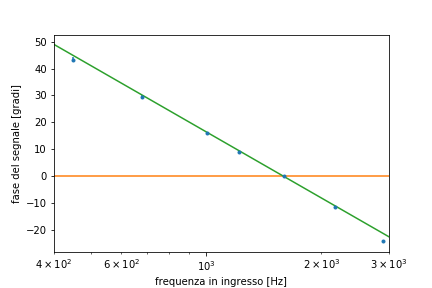
\includegraphics[width=\linewidth]{figure/1.png}
			\caption{sfasamento del segnale in funzione della frequenza in ingresso}
			\label{fig:1}
		\end{figure}
		\begin{figure}
			\centering
			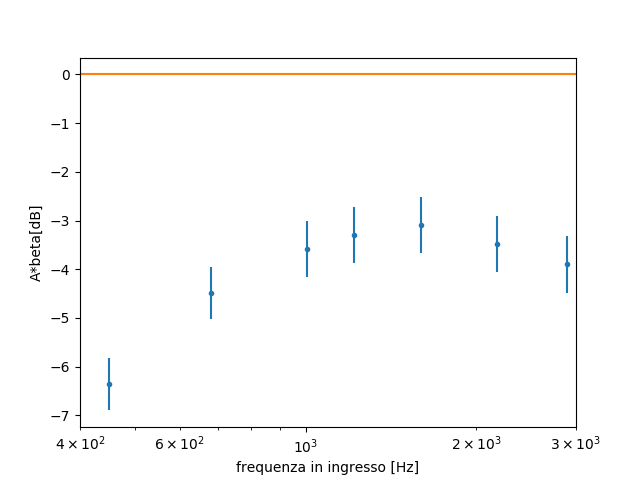
\includegraphics[width=\linewidth]{figure/2.png}
			\caption{Attenuazione del segnale in funzione della frequenza in infresso}
			\label{fig:2}
		\end{figure}
	\end{center}
	dalla figura \ref{fig:1} si evince chiaramente che lo sfasamento aumenta al diminuire della frequenza e si ha uno zero alla frequenza di taglio $f_t=1/2\pi\sqrt{R_1R_2C_1C_2}$, dove $R_1,R_2,C_1,C_2$ sono quelle indicate nel circuito in figura \ref{fig:circ1}
	\begin{figure}
		\centering
		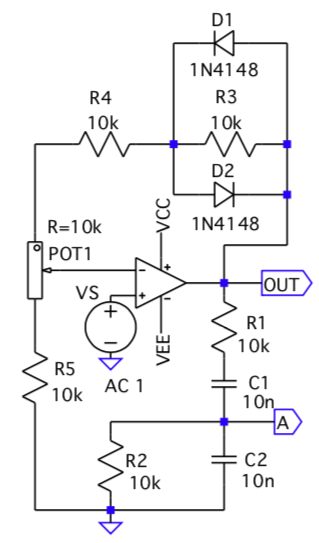
\includegraphics[width=\linewidth]{figure/circ1.png}
		\caption{Circuito 1}
		\label{fig:circ1}
	\end{figure}
	

\end{document}